\documentclass[twocolumn]{rbef}
\usepackage{lipsum}

\usepackage{bbm}
\usepackage{subfig}

\newcommand{\1}{\mathbbm{1}}
\newcommand{\s}{\mathcal{S}}
\newcommand{\T}{\mathcal{T}}
\newcommand{\A}{\mathcal{A}}
\newcommand{\ket}{\rangle}
\newcommand{\bra}{\langle}

\newtheorem{defi}{Definição}
\newtheorem{theorem}{Teorema}
\newtheorem{acknowledgement}[theorem]{Acknowledgement}
\newtheorem{algorithm}[theorem]{Algorithm}
\newtheorem{axiom}[theorem]{Axiom}
\newtheorem{claim}[theorem]{Claim}
\newtheorem{conclusion}[theorem]{Conclusion}
\newtheorem{condition}[theorem]{Condition}
\newtheorem{conjecture}[theorem]{Conjecture}
\newtheorem{corollary}[theorem]{Corollary}
\newtheorem{criterion}[theorem]{Criterion}
\newtheorem{definition}[theorem]{Definition}
\newtheorem{example}[theorem]{Example}
\newtheorem{exercise}[theorem]{Exercise}
\newtheorem{lemma}[theorem]{Lemma}
\newtheorem{notation}[theorem]{Notation}
\newtheorem{problem}[theorem]{Problem}
\newtheorem{proposition}[theorem]{Proposition}
\newtheorem{remark}[theorem]{Remark}
\newtheorem{solution}[theorem]{Solution}
\newtheorem{summary}[theorem]{Summary}
\newenvironment{proof}[1][Proof]{\noindent\textbf{#1.} }{\ \rule{0.5em}{0.5em}}

\titulocabecalho{Nostradamus: plataforma de aprendizado de máquina como um serviço para tratamento, análise, visualização e previsão de séries temporais providas pelo usuário}
\autorcabecalho{J. T. Anchante e A. R. A. Grégio}

\numeracao{01}
\volume{01}
\numero{01}
\ano{2019}
\doi{http://dsbd.leg.ufpr.br/tcc}
% \tipodeartigo{TCC DSBD}
\tipodeartigo{Especialização em Data Science \& Big Data}
% \addtocounter{page}{566} %% \setcounter produces extra white page!!! use ===\addtocounter===

\author[1]{Jayme T. Anchante}

\affil[1]{Departamento de Estatística, Universidade Federal do Paraná
  R. Evaristo F. Ferreira da Costa, 393 - Centro Politécnico, Jardim das Américas, 81531-990, Curitiba, PR, Brasil
  Brasil\thanks{\href{emailto:jayme.anchante@disroot.org}{jayme.anchante@disroot.org}}
}

\author[2]{André R. A. Grégio}

\affil[2]{Departamente de Informática, Universidade Federal do Paraná
  Rua Cel. Francisco Heráclito dos Santos, 100 – Centro Politécnico, Jardim das Américas, 81531-980, Curitiba,
  PR, Brasil\thanks{\href{emailto:gregio@ufpr.br}{gregio@ufpr.br}}
}

\titulo{Nostradamus: plataforma de aprendizado de máquina como um serviço para tratamente, análise, visualização e previsão de séries temporais providas pelo usuário}

\subtitulo{Nostradamus: machine learning as a service platform for treatment, analysis, visualization and prediction of time series provided by the user}

% -----------------------------------------------------------------------

\begin{document}

\begin{primeirapagina}

  % \begin{center}
  %   \vspace{-12pt} \small{Recebido em xxx. Aceito em xxx}
  % \end{center}

  \begin{abstract}
    O presente trabalho apresenta uma proposta de sistema automatizado de previsão de séries temporais chamado Nostradamus. Inicia-se o trabalho apresentando os principais conceitos de séries temporais, principais características e formas de tratamento. Em seguida, expôs-se o que se chamou de abordagem da estatística inferencial e de abordagem da estatística preditiva e as formas de tratamento e previsão de séries temporais de cada uma. Posteriormente, propôs-se o sistema automatizado Nostradamus, discutindo a forma de otimização e as etapas que o sistema percorre para alcançar a previsão final. No benchmark em sete bases de dados de séries temporais, o sistema Nostradamus alcançou o melhor resultado em cinco delas.
    \palavraschave{aprendizado de máquina, automl,
      séries temporais}

  \end{abstract}

  \begin{otherlanguage}{english}

    \begin{abstract}
      The present work presents a proposition of automated time series forecasting system called Nostradamus. First we introduce the main concepts of time series, main characteristics e treatments. Afterwards, we discuss what we called inferential statistics and predictive statistics approaches and the way each treat and forecast time series. Then, we propose the automated Nostradamus system, discussing the optimization and the steps the system make to reach the final forecast. In the benchmark with seven time series databases, the Nostradamus system reached the best result in five of them.
      \keywords{machine learning, automl,
        time series}

    \end{abstract}
  \end{otherlanguage}

\end{primeirapagina}
\saythanks

\section{Introdução} \label{intro}


Série temporal são dados pontuais ordenados temporalmente. Apesar do tempo ser contínuo, normalmente uma série temporal envolve dados discretos, tomados em sequência de períodos igualmente espaçados e sucessivos de tempo. Além da análise de séries temporais, ou seja, métodos para extrair estatísticas úteis e outras características dos dados, outro tema bastante relevante e objeto de estudos do presente trabalho é a predição de séries temporais, processo que envolve o uso de modelos que predigam valores futuros com base em valores passados observados.

A previsão de séries temporais é um tema bastante relevante e comum na vida de todos. Indivíduos verificam a previsão do tempo do dia seguinte para saber como se agasalhar ou se devem levar um guarda chuva, lemos no jornal a previsão da inflação para os próximos meses ou a cotação do dólar futuro, planejamos quanto iremos gastar por mês ao longo do ano ou até dos anos seguintes. Governos precisam prever os gastos do ano seguinte para ajustar o provimento do orçamento, prever o crescimento dos demais países para avaliar um acordo de comércio e o Banco Central deve prever a inflação dos próximos meses para fazer um ajuste na taxa de juros básica da economia. Empresas devem prever o demanda por seus produtos no varejo para que as lojas não fiquem desabastecidas, prever a sua receita nos próximos anos para avaliar um potencial investimento e exportadoras prevêem o dólar para que não incorram em prejuízos cambiais.

Séries temporais diferenciam-se de estudos de seção cruzada, pois estes não possuem nenhuma ordenação no tempo, como por exemplo o efeito da educação no salário dos indivíduos, em que os dados de diferentes pessoas podem ser colocados em qualquer ordem sem que haja prejuízo para a modelagem, ou ainda os dados são reflexo de um certo período de tempo, como por exemplo um censo decenal ou uma pesquisa anual. Diferenciam-se ainda de dados espaciais, pois estes possuem uma dependência geográfica, por exemplo o preço de imóveis depende da localização assim como de variáveis intrínsecas dos imóveis.

A análise de séries temporais pode ser dividia entre dois domínios: de frequência e de tempo. O último envolve o uso de funções matemáticas  ou sinais com respeito a frequência, ou seja, o quanto do sinal fica entre cada banda de frequência ao longo de uma série de frequências, algumas das transformações matemáticas mais utilizadas são as transformações de Fourier, de Laplace, Z e de Ondas, com aplicações em ondas sonoras, circuitos eletrônicos, processamento de sinal digital e compressão de dados. O domínio do tempo envolve o uso de funções matemáticas ou sinais com respeito ao tempo, que serão tratadas ao longo do presente trabalho.

Ainda, as técnicas de séries temporais podem ser divididas entre paramétricas e não paramétricas. As paramétricas assumem que os dados possuem um estrutura que pode ser descrita por um certo número finito (e normalmente pequeno) de parâmetros, que serão estimados para descrever o processo gerador dos dados, abordagem proposta pelo presente estudo. As técnicas não paramétricas tentam estimar diretamente os diferentes momentos dos dados (como média, variância e covariância) sem que seja assumido que o processo gerador possua qualquer estrutura em particular.

Por fim, a análise pode ser feita de forma univariada ou multivariada. O caso univariado trata de apenas uma série temporal, única e exclusivamente, enquanto que no caso multivariado, uma ou mais variáveis que podem ter uma relação de dependência são analisadas simultaneamente. Trataremos apenas do caso univariado.


O presente trabalho está organizado como se segue: analisaremos a forma como a estatística inferencial e como a estatística preditiva modelam séries temporais nas seções \ref{inferential} e \ref{predictive}, respectivamente, além de uma introdução de cada abordagem, cada seção também disporá de subseções que tratarão dos principais modelos utilizados assim como as medidas de sucesso de cada abordagem. A seção \ref{nostradamus} mostrará o funcionamento do sistema proposto Nostradamus, a função objetivo que o sistema minimiza, o algoritmo iterativo de busca de parâmetros, os algoritmos implementados e a estratégia de validação e previsão do sistema. A seção \ref{benchmark} mostrará um benchmark das duas abordagens realizando previsões em sete bases de dados com comportamentos e contextos distintos.

\section{Abordagem da estatística inferencial} \label{inferential}

O presente trabalho descreverá na presente seção a abordagem da estatística inferencial. Chamamos assim o conjunto de escolas, pensamentos, autores e paradigmas que tratam séries temporais utilizando modelos lineares, com validação do ajuste dentro da amostra, com foco principalmente, mas não exclusivamente, em testes de hipóteses, derivação de estimativas, dedução das propriedades da distribuição de probabilidades da série e generalização das conclusões para a população. Nesta seção apresentaremos as principais ideias deste \textit{corpus} representado por autores como Brockwell e Davis\cite{Brockwell}, Enders\cite{Enders}, Greene\cite{Greene}, Gujarati e Porter\cite{Gujarati}, Hayashi\cite{Hayashi}, Hamilton\cite{Hamilton}, Hyndman e Athanasopoulos\cite{Hyndman}. Seguiremos as discussões conforme o livro texto de Gujarati e Porter \cite{Gujarati}

Um dos grandes fundamentos da abordagem estatística é a natureza não determinística de séries temporais, ou seja, não podemos prever com total certeza valores futuros. Geralmente assume-se que uma série temporal ${x(t),t=0,1,2,...}$ segue um certo modelo de probabilidade que descreve a distribuição conjunta de uma variável aleatória $x_{t}$. A expressão matemática que descreve a estrutura de probabilidade de uma série temporal é chamada de processo estocástico. A sequência de observações da série na verdade é a realização de uma amostra do processo estocástico que a produziu.

\subsection{Estacionariedade, ruído branco e passeio aleatório} \label{stationary}

Uma característica importante de uma série temporal é a estacionariedade. Diz-se que um processo estocástico é estacionário se a média e a variância são constantes ao longo do tempo e o valor da covariância entre dois períodos depende exclusivamente da distância entre os dois períodos e não do período em que a covariância é computada. Esta definição é chamada de fracamente estacionária ou estacionária de covariância. Matematicamente, estacionariedade pode ser definida como:

\begin{equation}
E(Y_{t}) = u 
\gamma_{k} = E[(Y_{t} - u) (Y_{t+k - u})]
\end{equation}

\begin{equation}
var(Y_t) = E(Y_{t} - u)^2 = \sigma^{2} 
\end{equation}

\begin{equation}
\gamma_{k} = E[(Y_{t} - u) (Y_{t+k - u})]
\end{equation}

em que $\gamma_{k}$, a covariância na defasagem $k$, é a covariância entre os valores $Y_{t}$ e $Y_{t+k}$.

Se uma série temporal não atende os requisitos acima dizemos que ela é não estacionária. Séries temporais que exibem uma tendência ou sazonalidade são exemplos de séries não estacionárias (trataremos destes casos ao longo do texto). A estacionariedade é importante para questões de generalização: se a série é estacionária podemos extrapolar previsões para outros períodos além da série em questão com maior grau de precisão.

Um tipo especial de processo estocástico é o ruído branco ou puramente aleatório. Um processo é puramente aleatório se possuir média zero, variância constante e for serialmente não correlacionado. Ainda, se os valores forem independentes e identicamente distribuídos de uma distribuição normal, este processo é chamado de ruído branco Gaussiano.

Um exemplo de série temporal não estacionária é o passeio aleatório. Alguns dos exemplos práticos que seguem esse processo são os preços das ações, taxas de câmbio, preço de \textit{commodities}. Supondo um ruído branco $u_{t}$ com média zero e variância $\sigma^{2}$. Então $Y_{t}$ é um passeio aleatório se

\begin{equation}
Y_{t} = \delta + Y_{t-1} + u_{t}
\end{equation}

Assim, no modelo do passeio aleatório, o valor da série em um período qualquer $Y_{t}$ depende de um parâmetro delta $\delta$, conhecido como \textit{drift} - pois o parâmetro impulsiona a série para cima ou para baixo dependendo de seu sinal, do valor no período inicial $Y_{0}$ mais o valor dos choques aleatórios acumulados até o período $\sum u_{t}$, conhecido como tendência estocástica.

Podemos reescrever o modelo do passeio aleatório como sendo

\begin{equation} \label{unit_root_eq}
    Y_{t} = \rho Y_{t-1} + u_{t} \qquad -1 \leq \rho \leq 1
\end{equation}

Se $\rho = 1$, temos um modelo do passeio aleatório sem drift, também conhecido como problema de raiz unitária. Sabemos que o passeio aleatório é não estacionário, assim os termos passeio aleatório, não estacionariedade, raiz unitária e tendência estocástica podem ser tratados de forma sinônima. Se $|\rho| \leq 1$, então a série $Y_{t}$ é estacionária.

O conceito de passeio aleatório é um caso específico de uma classe mais abrangente de processos estocásticos chamada de processos integrados. O passeio aleatório é não estacionário, mas se tomarmos sua primeira diferença o processo se torna estacionário, assim ele é um processo integrado de ordem 1 ou $I(1)$. Ainda, uma série temporal que necessite ser diferenciada duas vezes é chamada de integrada de ordem 2. Em geral, se uma série necessita ser diferenciada \textit{d} vezes para ser estacionária, dizemos é integrada de ordem \textit{d}, denotada por $Y_{t} \sim I(d)$.


\subsection{Regressão espúria} \label{spurious}

Considerando duas variáveis aleatórias que seguem um processo do tipo passeio aleatório $Y_{t}$ e $X_{t}$ dependentes de ruídos brancos independentes e serialmente não correlacionados $u_{t}$ e $v_{t}$, respectivamente. Uma regressão entre estas variáveis produzirá coeficientes betas estatisticamente significativos, pois os testes usuais de significância são inválidos nestes casos\cite{Granger-Newbold}. Ainda, o coeficiente de determinação se mostra extremamente baixo, além de que a estatística $d$ de Durbin-Watson sugerir uma alta autocorrelação de primeira ordem\cite{Greene}. Este é o fenômeno da regressão espúria \cite{Yule}.

Regressões deste tipo não possuem nenhum significado, o que pode ser atestado quando realizamos a mesma regressão, entretanto com ambas as variáveis em suas primeiras diferenças, deixando-as estacionárias. O coeficiente de determinação ficará perto de zero, e a estatística de Durbin-Watson estará próxima de 2.

\subsection{Testes de raiz unitária} \label{unit_root}

Supondo um processo do tipo estocástico de raiz unitária como da equação \ref{unit_root_eq}. Se $\rho = 1$, temos o modelo do passeio aleatório sem drift, portanto um processo não estacionário. Entretanto, não podemos estimar diretamente o parâmetro $\rho$ para verificar se o coeficiente é igual a 1, pois o teste $t$ de Student fica viesado no caso de raiz unitária. Mas podemos subtrair $Y_{t-1}$ de ambos os lados da equação, assim

\begin{equation} \label{Dickey_Fuller_eq}
    \Delta Y_{t} = \delta Y_{t-1} + u_{t}
\end{equation}

em que $\delta = (1-\rho)$ e $\Delta$ é o operador da primeira diferença. Sob a hipótese nula de que $\delta = 0$ (contra a hipótese alternativa de que $\delta < 0$), a estatística \textit{t} segue a distribuição $\tau$\cite{Dicker-Fuller}, assim este teste é conhecido como teste de raiz unitária de Dickey-Fuller. A equação \ref{Dickey_Fuller_eq} pode ainda ser reespecificada incluindo um \textit{drift} na forma de um $\beta_{1}$ ou ainda incluindo o \textit{drift} e uma tendência determinística $\beta_{2}t$. Uma segunda versão chamada de teste de Dickey-Fuller aumentado inclui defasagens da variável dependente $\Delta Y_{t-i}$ para tentar capturar autocorrelações de maior grau.

Existem outros testes para detectar a presença de uma raiz unitária em uma série temporal. O teste desenvolvido por Elliot, Rothenberg e Stock\cite{Elliot-Rothenberg-Stock} conhecido como ADF-GLS é assintoticamente mais indicado que o teste usual de Dickey-Fuller caso a especificação tenha \textit{drift} e/ou tendência determinística. O teste de Phillips-Perron\cite{Phillips-Perron} leva em consideração uma possível autocorrelação no termo de erro ao se introduzir defasagens da variável dependente. O teste KPSS de Kwiatkowski–Phillips–Schmidt–Shin\cite{Kwiatkowski} testa a hipótese nula de que a série é estacionária ao redor de uma tendência determinística contra a hipótese alternativa de raiz unitária.

\subsection{Modelos de séries temporais} \label{arima}

Os tipos de modelos de séries temporais podem ser classificados em aproximadamente cinco tipos\cite{Gujarati}: i) métodos de suavização, que consistem em ajustar uma curva suave em dados históricos\cite{Hyndman}, tais como os métodos de suavização exponencial\cite{Brown}, Holt linear\cite{Holt}, Holt-Winters\cite{Winters}, entre outros; ii) modelos de regressão de uma única equação, como o caso de prever a demanda de um determinado produto com base nos preços do produto, preços de produtos concorrentes e complementares, renda dos consumidores e outros fatores; iii) modelos de regressão de equações múltiplas, várias equações são especificadas para tentar capturar a influência dos diversos fatores em uma previsão, assim como a influência de uma previsão em outros fatores; iv) modelos baseados na metodologia de Box e Jenkins\cite{Box-Jenkins}, tecnicamente conhecidos como modelos \textit{ARIMA}, que trataremos mais na presente seção, analisam as propriedades estocásticas utilizando valores passados da uma série para tentar explicar valores presentes/futuros; v) modelos de vetores autorregressivos, sistema de multiequações em que valores das variáveis endógenas são explicados por valores passadas das mesmas variáveis e passados das outras variáveis endógenas.

Desenvolveremos os principais conceitos do modelo \textit{ARIMA} por ser um dos modelos mais utilizados dentro da chamada abordagem inferencial dentro de um contexto preditivo. Seja $Y_{t}$ uma série temporal, podemos modelá-la como

\begin{equation}
    (Y_{t} - \delta) = \alpha_{1} (Y_{t-1} - \delta) + u_{t}
\end{equation}

em que $\delta$ é a média de $Y$ e $u_{t}$ é um ruído branco, podemos dizer que $Y_{t}$ segue um processo autorregressivo de primeira ordem ou \textit{AR(1)}, por ser incluída uma defasagem de $Y$ como variável explicativa. Caso $Y$ dependa de \textit{p} defasagens dizemos que segue um processo autorregresivo de ordem \textit{p} ou \textit{AR(p)}, assim no caso mais geral temos

\begin{equation}
    (Y_{t} - \delta) = \alpha_{1} (Y_{t-1} - \delta) + \alpha_{2} (Y_{t-2} - \delta)+ ... + \alpha_{p} (Y_{t-p} - \delta) + u_{t}
\end{equation}

Um outro possível processo gerador de $Y_{t}$ pode ser a seguinte distribuição

\begin{equation}
    Y_{t} = \mu + \beta_{0} u_{t} + \beta_{1} u_{t-1}
\end{equation}

em que $\mu$ é uma constante e $u$ é o termo de erro que segue um processo do tipo ruído branco. Aqui o termo $Y_{t}$ depende de uma constante mais a média móvel dos termos presentes e passados, assim neste caso temos um modelo de média móvel de primeira ordem ou \textit{MA(1)}. De forma mais geral temos

\begin{equation}
    Y_{t} = \mu + \beta_{0} u_{t} + \beta_{1} u_{t-1} + \beta_{2} u_{t-2} + ... + \beta_{q} u_{t-q}
\end{equation}

Temos que $Y_{t}$ segue um processo de média móvel de ordem \textit{q} ou \textit{MA(q)}. Em resumo, a media móvel é uma combinação linear dos termos de erro, que são ruídos brancos.

Uma variável aleatória $Y$ pode conter processos autorregressivos de ordem \textit{p} e de médias móveis de ordem \textit{q}, neste caso temos um processo do tipo \textit{ARMA(p, q)}. Caso a variável em questão seja não estacionária, deve-se tomar a diferença dela até que ela atinja a estacionariedade, assim o processo pode ainda ter um componente integrado de ordem \textit{d} ou \textit{I(d)}, neste caso temos o modelo \textit{ARIMA(p, d, q)}. Dentro da metodologia de Box-Jenkins\cite{Box-Jenkins} a série deve ser necessariamente estacionária para que se possam fazer previsões além do período da amostra. Assim, dado que $Y_{t}$ é uma série que precisou de \textit{d} diferenças para se tornar estacionária, podemos representar o modelo ARIMA como

\begin{equation}
    Y_{t} = \theta + \sum_{1}^{p} \alpha_{p} Y_{t-p} + \beta_{0} u_{t} + \sum_{1}^{q} \beta_{q} u_{q}
\end{equation}

em que o processo possui zero ou mais componentes autorregressivos, um termo de erro presente do tipo ruído branco e zero ou mais components de médias móveis, sendo $\theta$ o termo constante. A metodologia de Box-Jenkins\cite{Box-Jenkins} consiste em quatro etapas: i) identificação dos parâmetros \textit{p}, \textit{d} e \textit{q}; ii) estimação dos parâmetros; iii) checagem e validação dos resultados; iv) caso o modelo seja validado, podemos prosseguir para a previsão de valores futuros. A seguir discutiremos um pouco de cada uma destas etapas.

A primeira parte na identificação dos parâmetros é garantir que a série seja estacionária, para isso podem ser realizados um ou mais dos testes discutidos na seção \ref{unit_root}. Assim que a série for estacionária, podemos proceder a identificação dos parâmetros \textit{p} e \textit{q} utilizando correlogramas. O correlograma de função de autocorrelação (ACF) mede a correlação entre uma variável aleatória e uma de suas defasagens no período $k$. O correlograma de função parcial de autocorrelação (PACF) mede a correlação entre uma variável aleatória e uma de suas defasagens no período $k$, mas controlando por todas as defasagens entre o momento presente $t$ e a defasagem $k$. De maneira geral, um processo \textit{AR(p)} decai exponencialmente no ACF e possui picos até a defasagem \textit{p}, um processo \textit{MA(q)} decai exponencialmente no PACF e possui picos até a defasagem \textit{q} e um processo \textit{ARMA(p, q)} decai exponencialmente em ambos os correlogramas.Note que o processo de identificação muitas vezes é mais uma arte que um processo completamente objetivo\cite{Enders}.

A estimação do modelo \textit{ARIMA(p, d, q)} pode ser feita via método de Mínimo Quadrados Ordinários. Para diagnóstico do modelo, podemos utilizar os resíduos da regressão e realizar os testes de raiz unitária mencionados na seção \ref{unit_root} e ainda realizar os testes de autocorrelação serial de Box-Pierce\cite{Box-Pierce} ou de Ljung-Box\cite{Ljung-Box}. Ainda, poderiam ser utilizados os critérios de informação para seleção de modelos com diferentes configurações de parâmetros, assim quanto menor o valor do critérios de informação mais parcimoniosos são os modelos e melhor a qualidade do ajuste. Por exemplo, o critério de informação de Akaike\cite{Akaike} conhecido como AIC em que o valor depende diretamento do número de parâmetros incluídos no modelo e inversamente proporcional ao valor da máxima verossimilhança. O critério de informação de Schwarz\cite{Schwarz} é conhecido como BIC por ter sido feito um argumento Bayesiano no artigo seminal de Schwarz, ele depende diretamento do número de amostras e do número de parâmetros e inversamente da máxima verossimilhança. O critério de Hannan-Quinn\cite{Hannan} conhecido como HQ depende do número de parâmetros e do número do valor de amostras duplo \textit{log}, garantindo consistência do critério, e inversamente proporcional a máxima verossimilhança.

\begin{equation}
    \begin{split}
        & AIC = 2k + 2 \ln (\hat{L}) \\
        & BIC = \ln (n) k - 2 \ln (\hat{L}) \\
        & HQ = -2 L_{max} + 2k \ln (\ln (n)) \\
    \end{split}
\end{equation}

Com um modelo com erros estacionários e não serialmente autocorrelacionados e com baixo valor nos critérios de informação frente a outros modelos, podemos realizar previsões \cite{Hamilton} de valores que extrapolem o período da amostra da série temporal. Note ainda que o modelo \textit{ARIMA} pode ser extendido dependendo das condições da série temporal, tais como sazonalidade ou heteroscedasticidade condicional\cite{Brockwell}, apesar de não ser o foco do presente trabalho. A seguir trataremos da outra abordagem de séries temporais que tem foco na análise preditiva.

\section{Abordagem da estatística preditiva} \label{predictive}

A abordagem da estatística preditiva refere-se ao fato de que o objetivo principal e fundamental desta abordagem é a previsão de valores além dos estabelecidos pela amostra, e, no caso de séries temporais, de valores futuros posteriores ao limite do período da amostra. A instrumentação desta abordagem é a de técnicas de validação cruzada, modelos não lineares, métricas de avaliação por meio do erro da previsão e tomadas fora da amostra em que o modelo foi treinado, com relaxamento da maioria das hipótese tratadas na seção \ref{inferential}. Aprofundaremos a discussão de alguns conceitos iniciais introdutórios.

Inteligência artificial (AI) é a inteligência exibida pelas máquinas - contrastando com a inteligência natural dos humanos - que pode ser implementada por meio de regras pré determinadas por humanos ou por meio de padrões aprendidos com dados históricos, caso do aprendizado de máquina\cite{Oliver}. A maioria dos sistemas de inteligência artificial exibe apenas características de inteligência cognitiva, ou seja, conhecimento por meio de pensamento, experiência ou sentidos. Cada sistema de inteligência artificial tende a focar em uma tarefa específica do conhecimento, chamado de AI aplicada, como por exemplo processamento de linguagem natural, visão computacional, sistemas de detecção de doenças, entre outros, entretanto um dos objetivos de longo prazo é alcançar a chamada inteligência generalista, capaz de exercer uma gama de tarefas cognitivas aplicando uma série de resoluções de problemas\cite{Laird}.

Aprendizado de máquina (ML) é o estudo de modelos estatísticos utilizados de forma a realizar uma determinada tarefa efetivamente sem colocar instruções pré definidas\cite{Samuel}. O conjunto de regras são inferidas a partir de padrões aprendidos por meio de dados históricos da tarefa em questão. Pode ser dividida em três grupos: i) aprendizado supervisionado, em que existem características que são utilizadas para prever uma variável alvo, caso o alvo seja uma variável contínua é dito que o problema é de regressão, caso o alvo seja uma categoria é dito que o problema é de classificação; ii) não supervisionado, em que não existe um alvo propriamente dito a ser previsto, mas o problema consiste em encontrar padrões nos dados, no caso da \textit{clusterização} é agrupando as amostras similares entre si, no caso da redução de dimensionalidade é reduzir o número de características de forma a manter a maior variabilidade/ortogonalidade dos dados; iii) aprendizado por reforço, em que os algoritmos recebem o \textit{feedback} de acordo com suas ações em um ambiente normalmente simulado e dinâmico, muito utilizado no caso de carros autônomos e aprendizado de jogos de tabuleiro e virtuais.

A seguir apresentaremos alguns dos principais algoritimos utilizados em aprendizado de máquina. Posteriormente, apresentaremos o tratamento do sistema proposta para a previsão de séries temporais.

\subsection{Algoritmos preditivos} \label{algos}

O primeiro algoritmo que iremos discutir é o mesmo utilizado na seção \ref{arima} que é a Regressão Linear. Neste caso tentamos prever uma variável alvo $y$ que é um vetor coluna em função de uma matriz $X$ composta de $n$ características\cite{Greene}, como

\begin{equation}
    y_{i} = \beta_{0} + \beta_{1} x_{i1} + \beta_{2} x_{i2} + ... + \beta_{n} x_{in} + \epsilon_{i}
\end{equation}

em que $\epsilon$ é o termo de erro que captura todas as relações não lineares ou das variáveis omitidas no modelo. A estimação é feita via método de mínimos quadrados ordinários em que a função objetivo soma quadrada dos resíduos (SQR) deve ser minimizada encontrando os parâmetros $\beta$ ótimos

\begin{equation}
    SQR = \sum_{i=1}^{N} (y_{i} - \hat{y_{i}})^{2}
\end{equation}

em que $y_{i}$ é o valor da observação de fato e $\hat{y_{i}}$ é o valor da observação previsto pelo modelo.

O primeiro algoritmo não linear que trataremos é $k$ Vizinhos Próximos. É um algoritmo do tipo baseado em aprendizado de instâncias ou aprendizado preguiçoso - já que é baseado em memória e não necessita que nenhum modelo seja ajustado. Dado um novo ponto $k_{0}$, encontra-se os $k$ pontos $x_{r}, r=1,...,k$ de treinamento mais próximos em distância a $x_{0}$ e atribuímos um valor ao novo ponto usando algum tipo de média. Assumindo que as características tem valores reais\cite{Hastie}

\begin{equation}\label{euclidian}
    d_{i} = \| x_{i} - x_{0} \|
\end{equation}

podemos utilizar a distância euclidiana da equação \ref{euclidian}. Tipicamente padronizamos cada uma das características para que tenham escalas similares. Quando utilizamos $k=1$ - apenas o vizinho mais próximo - temos um sistema com viés baixo mas uma variância elevada, situação que vai ficando menos acentuada a medida que acrescentamos mais vizinhos.

Árvores de Decisão separam a base de dados no primeiro nó, chamado de raiz, em conjuntos menores, chamados de nós filhos, que juntos compõe um galho, até o momento em que uma nova separação não adicione valor a previsão. Algoritmos geralmente funcionam de "cima para baixo", escolhendo a cada etapa a variável que fará a melhor separação. A métrica do que é melhor é uma medida de homogeneidade da variável alvo dentro dos conjuntos.

Uma destas medidas é o Coeficiente de Impureza de Gini que mede o quão frequentemente uma amostra aleatória estaria no conjunto errado se fosse predita de acordo com a distribuição do alvo neste conjunto. Outra medida é o Ganho de Informação ou divegência de Kullbrack-Leibler\cite{Kullbrack} mede a quantidade de informação ganha sobre o alvo ao utilizar uma das características para separação calculando a entropia do nó pai substraído da soma dos nós filhos ponderados.

De forma geral, podemos representar o modelo de Árvore de Decisão como\cite{James}

\begin{equation}
    f(X) = \sum_{m=1}^{M} c_{m} \cdot 1_{(X \in R_{m})}
\end{equation}

em que $R_{1}, ..., R_{m}$ representam partições do espaço de características. Árvores de Decisão são estimadores chamados de "fracos", mas que quando utilizados em conjunto podem ter um grande poder preditivo. Algumas das técnicas para agrupamento destes estimadores são \textit{Bagging}\cite{BreimanBag} - em que cada Árvore de Decisão recebe um subconjunto dos dados e a previsão final é uma média de todos os estimadores, \textit{Florestas Aleatórias}\cite{BreimanRF} - em que cada Árvore recebe um subconjunto dos dados e um subconjunto das características, \textit{Boosting}\cite{BreimanB} - consiste em encadear uma série de Árvores de Decisão de forma com que cada estimador seja ajustado nos erros do estimador anterior, aprendendo de forma gradual os padrões dos dados.

Máquinas de vetor de suporte é um algoritmo que representa os dados como pontos de um espaço vetorial, separado-os por meio de um ou um conjunto de hiperplanos de tal forma que as diferentes classes fiquem separadas de forma ótima e o mais distantes possível\cite{Cortes}. Além de poder mapear relações lineares entre as variáveis, utilizando o chamado truque do \textit{kernel}\cite{Aizerman} é possível capturar relações não lineares mapeando as características para espaços dimensionalmente mais elevados.

Caso os dados sejam linearmente separáveis, pode definir um hiperplano de suporte $\vec{w} \cdot \vec{x_i} - b$, em que dados acima deste hiperplano pertencem a uma classe, e pontos abaixo pertencem a outra classe. Caso os dados não sejam linearmente separáveis, podemos introduzir a função do tipo \textit{hinge loss} que é do tipo $max(0, 1 - \vec{w} \cdot \vec{x_i} - b)$, ou seja, zero caso o vetor $\vec{x_{i}}$ fique do lado correto da margem. Para dados do lado incorreto da margem, o valor da função é proporcional a distância da margem. Assim desejamos minimizar

\begin{equation}
    \Bigg[ \frac{1}{n} \sum_{i=1}^{n} max(0, 1 - \vec{w} \cdot \vec{x_i} - b) \Bigg] + \delta \|\vec{w}\|^2
\end{equation}

que é a função \textit{hinge loss} para cada uma das amostras com um parâmetro $\delta$ que determina o \textit{trade-off} entre aumentar o tamanho da margem e garantir que o vetor $\vec{x_{i}}$ fique dentro do lado correto da margem.

Redes neurais artificiais são sistemas com estrutura inspirada nas redes neurais biológicas que constituem o cérebro. A rede neural é constituída por uma série de unidades ou nós chamados de neurônios artificiais que normalmente são completamente conectados entre si. Cada conexão transmiti o sinal de um neurônio para o outro, o neurônio que recebe o sinal é capaz de processá-lo e passá-lo aos neurônios seguintes conectados. Normalmente o sinal é um número real e o sinal enviado é um calculado por uma função não linear - conhecida como função de ativação - da soma dos sinais recebidos. As conexões entre os neurônios é chamada de aresta, os neurônios e as arestas tem um peso que é ajustado conforme o aprendizado avança, sendo que o peso pode aumentar ou reduzir o sinal numa conexão. Normalmente, os neurônios estão agrupados em camadas, sendo a primeira camada chamada de camada de entrada e a camada final a camada de saída\cite{James}. Redes neurais profundas fazem parte de uma classe de algoritmos conhecidos como aprendizado profundo, em contraste com o aprendizado raso descrito nos algoritmos anteriores, quando as redes neurais possuem camadas entre as de entrada e de saída - conhecidas como camadas escondidas - que atuam como extratoras de características dos dados brutos de entrada, retirando parte do problema do usuário de manualmente extrair características relevantes dos dados.

Uma rede neural pode ser entendida como um problema de duas etapas. As características derivadas $Z_{m}$ de combinações lineares dos dados de entrada, cada camada $T$ é uma combinação linear das características derivadas, os dados de saída são uma função linear da última camada escondida\cite{Hastie}

\begin{equation}
    \begin{split}
        & Z_{m} = \sigma (\alpha_{0m} + \alpha_{m}^{T} X  ), \qquad m=1,...,M \\
        & T_{k} = \beta_{0k} + \beta_{k}^{T}Z, \qquad k=1,...,K \\
        & f_{k}(X) = g_{k}(T), \qquad k=1,...,K
    \end{split}
\end{equation}

alguns tipos de funções de ativação $\sigma(v)$ normalmente escolhidos são sigmóide, base radial Gaussiana, retificação linear. A função de ativação na camada de saída $g_{k}(T)$ permite uma transformação final, que no caso da regressão é a função identidade. Alguns desafios no treinamento de redes neurais são a escolha dos valores iniciais dos pesos que pode impactar no otimização posterior, sobreajustamento nos dados ficando "viciado" nos dados de treinamento ao permanecer num mínimo local, escala dos dados de entrada pois uma característica numa escala maior pode acabar dominando as demais características, a escolha do número de camadas e número de neurônios por camada e finalmente diversos mínimos locais, não convergindo para um mínimo global\cite{Hastie}.

\subsection{Critérios de avaliação dos modelos} \label{subsection22}

Uma das etapas mais importantes para avaliação e validação de modelos é a separação e amostragem da base de dados. Existem várias estratégias se amostragem, incluindo \textit{bootstrap}, "deixar um de fora", validação cruzada com $k$ dobras, \textit{hold-out}. Independente da estratégia, usualmente os dados são divididos entre três partes: base de treinamento, base de validação, e base de teste\cite{James}.

A base de treinamento é utilizada para testar a performance de diversos algoritmos e diversas configurações de hiperparâmetros para cada algoritmo. A base de treinamento pode ser dividida utilizando uma das estratégias de subamostragem mencionadas anteriormentes para que o algoritmo não fique sobreajustado nestes dados e consiga generalizar frente a novos dados. Uma vez escolhido o algoritmo mais adequado com a melhor configuração de hiperparâmetros, podemos ajustá-lo em cima de toda a base de treinamento, mas verificando a performance dele a cada certa quantidade de iterações, épocas ou etapas de aprendizado na base de validação para garantir novamente que o modelo não acabe sobreajustando os dados de treinamento, utilizando um certo critério de parada que faça com que o algoritmo pare de aprender os padrões dos dados caso o erro de validação não caia mais.

A última etapa de verificação de performance do algoritmo consiste em fazer uma predição na base de teste, também chamada de conjunto \textit{hold-out}, já que são dados nunca antes vistos pelo algoritmo. Assim, tenta-se reproduzir um cenário em que novos dados cuja variável alvo é totalmente desconhecida devem ser preditos, a diferença sendo que neste teste controlado sabemos o real valor da variável alvo.

Discutiremos algumas das métricas de performance mais utilizadas no contexto de regressão. O Erro Absoluto Médio (MAE) é a diferença entre o real valor da variável alvo e o valor predito pelo modelo. O Erro Quadrático Médio é semelhante ao MAE, mas a diferença é elevada ao quadrado, penalizando predições com maior erro. O Erro Quadrático Logarítmico Médio (MSLE) toma o log dos valores tanto da variável alvo quanto das predições, assim a variância é medida numa escala logarítmica, é utilizada para não penalizar grandes diferenças entre os valores do alvo e os valores previstos, quando ambos estão em uma escala relativamente grande.

\begin{equation} \label{mineq}
    \begin{split}
        & MAE = \sum_{i=1}^{n} (y_{i} - \hat{y_{i}}) / n \\
        & MSE = \sum_{i=1}^{n} (y_{i} - \hat{y_{i}})^2 / n \\
        & MSLE = \sum_{i=1}^{n} (\log(1 + y_{i}) - \log(1 + \hat{y_{i}}))^2 / n \\
    \end{split}
\end{equation}

\section{Plataforma automatizada de predição de séries temporais Nostradamus} \label{nostradamus}

Após apresentar alguns dos principais conceitos das abordagens inferencial e preditiva em relação a séries temporais, iremos apresentar uma proposta de sistema automatizado de previsão de séries temporais que tenta unir conceitos de ambas as abordagens. Abstraindo o máximo possível as questões técnicas relativas ao tratamento de séries temporais, como o processamento dos dados, construção de características, modelagem, validação e previsão.

Todo o sistema pode ser definido numa função objetivo

\begin{equation}
    \begin{split}
        & \min \quad MAE = f(FE(p), Algo(HP)) \\
        & \text{tal que} \qquad p <= n / 20 \\
        & \qquad \qquad \quad Algo(HP) \to Data \\
    \end{split}
\end{equation}

em que o objetivo é minimizar o erro absoluto médio das previsões de acordo com uma função de $FE$, do inglês \textit{Feature Engineering}, ou Engenharia de Características e de um $Algo$ ou algoritmo que tem $HP$, do inglês \textit{hyperparameters}, ou hiperparâmetros. A primeira restrição significa que a ordem $p$ da engenharia de características não deve exceder a vigésima parte do número de dados da série temporal. Já a segunda restrição afirma que os hiperparâmetros específicos de um algoritmo devem satisfazer as restrições impostas pela base de dados (número de colunas, intervalo de valores etc).

Como engenharia de características, é feita uma transformação da série temporal em um processo autorregressivo \textit{AR(p)}

\begin{table}[!htb]
    \caption{Transformação dos dados em processo AR(p)}
    \begin{minipage}{.5\linewidth}
      \caption{Dados originais}
      \centering
        \begin{tabular}{ll}\label{rawdata}
            $t$ & $valor$ \\
            0 & 10 \\
            1 & 11 \\
            2 & 12 \\
            3 & 13 \\
            4 & 14 \\
            5 & 15 \\
            6 & 16 \\
            7 & 17 \\
            8 & 18 \\
            9 & 19 \\
        \end{tabular}
    \end{minipage}%
    \begin{minipage}{.5\linewidth}
      \centering
        \caption{Dados AR(2)}
        \begin{tabular}{lll}\label{AR2}
            $x_{t-2}$ & $x_{t-1}$ & $Y$ \\
            10 & 11 & 12 \\
            11 & 12 & 13 \\
            12 & 13 & 14 \\
            13 & 14 & 15 \\
            14 & 15 & 16 \\
            15 & 16 & 17 \\
            16 & 17 & 18 \\
            17 & 18 & 19 \\
        \end{tabular}
    \end{minipage} 
\end{table}

No caso da série temporal original na tabela \ref{rawdata}, temos que a primeira coluna $t$ é uma contagem dos períodos e a segundo coluna é o valor em si da série temporal. Na tabela \ref{AR2}, temos que as colunas $x_{t-2}$ e $x_{t-1}$ representam as defasagens 2 e 1, respectivamente, de um processo $AR(2)$, que também podem ser entendidos como as características ou dados de entrada do modelo, já a coluna $Y$ é a série temporal no tempo presente $t$, que também pode ser entendida como a variável alvo. Importante notar que a série temporal original possuía 10 linhas ou amostras, já os dados transformados possuem 8 linhas ou amostras. Se tivéssemos feito um processo do tipo $AR(3)$, os dados transformados possuiriam 7 linhas. Podemos dizer que há um \textit{trade-off} entre tamanho e profundidade da base de dados transformada: quanto maior o grau do processo $AR$, maior a capacidade de capturar padrões passados que podem ajudar a explicar os valores presentes da série temporal, contudo, menor a quantidade de dados disponíveis para o modelo treinar e aprender sobre da série.

Conforme exposta na seção \ref{algos}, cada algoritmo aprende os padrões dos dados de uma forma distinta, portanto certos algoritmos podem capturar mudanças que outros não o fariam, assim optou-se por implementar a maior gama de algoritmos preditivos possível para que o sistema escolha aquele que tem a melhor performance. Os algoritmos preditivos implementados pela plataforma são: regressão linear, \textit{elasticnet} (uma regressão linear com regularização L1 e L2), florestas aleatórias, $k$ vizinhos próximos, rede neural profunda, implementados pela biblioteca \textit{scikit-learn}\cite{Pedregosa}; um algoritmo de impulso de gradiente extremo baseado em árvore de decisão com \textit{boosting} chamado de XGBoost\cite{Chen}.

A forma de minimização de \ref{mineq} é feita por meio de um processo iterativo em que a cada etapa um valor de $p$ é escolhido para a engenharia de características, assim como um dos algoritmos mencionados anteriormente com uma configuração de hiperparâmetros amostrada de forma que faça sentido com os dados obedecendo a segunda restrição de \ref{mineq}. Este processo poderia ser feita de forma totalmente aleatória a cada iteração, o que faria com que a maior parte do espaço amostral possível fosse coberto dado que iterações suficientes sejam feitas. Entretanto, como os recursos computacionais são finitos, assim como o tempo total que o usuário final está disposto a esperar para que o sistema atinja a convergência, optou-se por utilizar um algoritmo de busca Bayesiana\cite{Lévesque}. Este algoritmo de busca funciona da seguinte maneira: inicialmente são feitas $x$ iterações amostradas de forma totalmente aleatória para que o sistema gere dados iniciais. As amostragens de parâmetros são as características que serão inputadas e o erro absoluto médio é a variável alvo do algoritmo Bayesiano, assim após $x$ iterações, o algoritmo começará a testar espaços amostrais mais promissores de forma mais consistente, mas mantendo a busca aleatória a cada $y$ iterações para que o sistema não caia em um mínimo local.

Adotou-se uma estratégia de separação da série temporal entre treinamento e teste. Noventa por cento da série é utilizada como dados de treinamento, que serão utilizados para o ajuste do algoritmo Bayesiano de otimização, numa estratégia de validação cruzada de quatro dobras, sendo que o erro absoluto médio de cada iteração é a média aritmética das quatro dobras. Após a seleção do melhor grau $p$ para a engenharia de características e do melhor algoritmo com a melhor configuração de hiperparâmetros encontrada, esta configuração global será ajusta na totalidade dos dados de treinamento e será feita uma previsão na mesma quantidade de passos a frente que os dez por cento da série separada como base de teste. Assim é possível calcular o erro absoluto médio de forma sequencial em uma base de dados totalmente independente, métrica que será reportada para o usuário final como sendo a métrica de performance geral do algoritmo. Após esta última etapa de validação, o algoritmo com a melhor configuração encontrada é ajustado na totalidade da série temporal e é feita a previsão $n$ passos a frente.

\subsection{Benchmark da plataforma em bases de dados} \label{benchmark}

Nesta seção mostraremos o resultado de um \textit{benchmark} de três \textit{frameworks} na previsão de 7 séries temporais. O primeiro \textit{framework} é a própria plataforma Nostradamus proposta no presente trabalho, o segundo é uma implementação em Python pela biblioteca \textit{pmdarima} da função \textit{auto.arima} da biblioteca \textit{forecast} de R, o terceiro é um algoritmo chamado de \textit{Prophet} baseado em simulação de Monte Carlo implementado pela biblioteca \textit{fbprophet}.

As séries temporais utilizadas como \textit{benchmark} são: \textit{sunspots}, número de manchas solares por ano entre 1700 e 2008; \textit{airpassengers}, número mensal de passageiros de vôos de avião; \textit{austres}, dados residenciais trimestrais; \textit{heartrate}, frequência cardíaca; \textit{lynx}, número de linces capturados por ano no Canadá entre 1821 e 1934; \textit{wineind}, vendas de vinho da indústria australiana; e \textit{woolynrnq}, produção trimestral de lã na Austrália. Foram separados os dez por cento dos pontos mais recentes de cada conjunto de dados como base de teste e cada \textit{framework} recebeu os noventa por cento de dados restantes para treinamento.

A seguir reportamos o erro absoluto médio de cada uma das bases de dados para cada um dos sistemas testados:

\begin{table}[!htb]
    \caption{Erro absoluto médio nos 10\% de cada série temporal utilizados para validação para a previsão de cada um dos três sistemas, Nostradamus, ARIMA e Prophet}
    \center
    \begin{tabular}{llll}
	    Base & Nostradamus & ARIMA & Prophet \\
	    sunspots & 18.93 & 44.41 & 45.50  \\
	    airpassengers & 88.74 & 39.35 & 57.93 \\
	    austres & 41.74 & 56.43 & 115.42  \\
	    heartrate & 1.64 & 2.01 & 2.16  \\
	    lynx & 198.49 & 652.95 & 967.96  \\
	    wineind & 5939.42 & 3817.89 & 3762.36  \\
	    woolnrq & 426.8 & 427.38 & 592.50  \\
    \end{tabular}
\end{table}


Vemos que o sistema Nostradamus teve o menor erro absoluto médio em 5 das 7 bases de dados, \textit{sunspots}, \textit{austres}, \textit{heartrate}, \textit{lynx}, \textit{woolnrq}. O modelo ARIMA teve o menor erro na base \textit{airpassengers}. O modelo \textit{Prophet} teve o menor erro na base \textit{wineind}. Nota-se que nas bases em que o sistema Nostramus não obteve o melhor resultado, seu erro foi consideravelmente mais elevado que os demais modelos. Para entender melhor o comportamento de cada previsão em relação a série temporal que ocorreu de fato, mostram-se duas figuras, a primeira em que Nostradamus obteve o melhor resultado, enquanto na segunda ele teve a pior performance

\begin{figure}[!htb]
	\centering 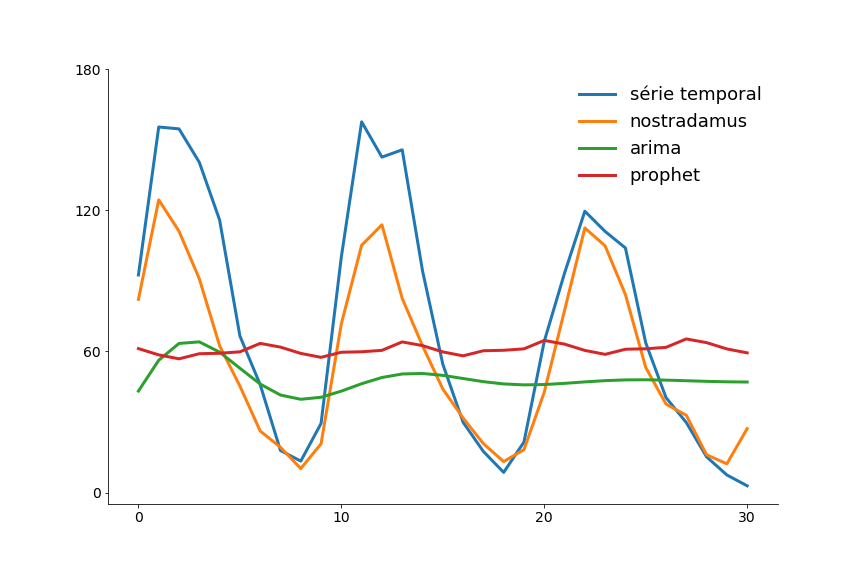
\includegraphics[scale=0.3]{fig1.png}
	\caption{Previsão de cada sistema na base \textit{sunspots} nos 10\% da base reservados para teste}
	\label{fig1}
\end{figure}

\begin{figure}[!htb]
	\centering 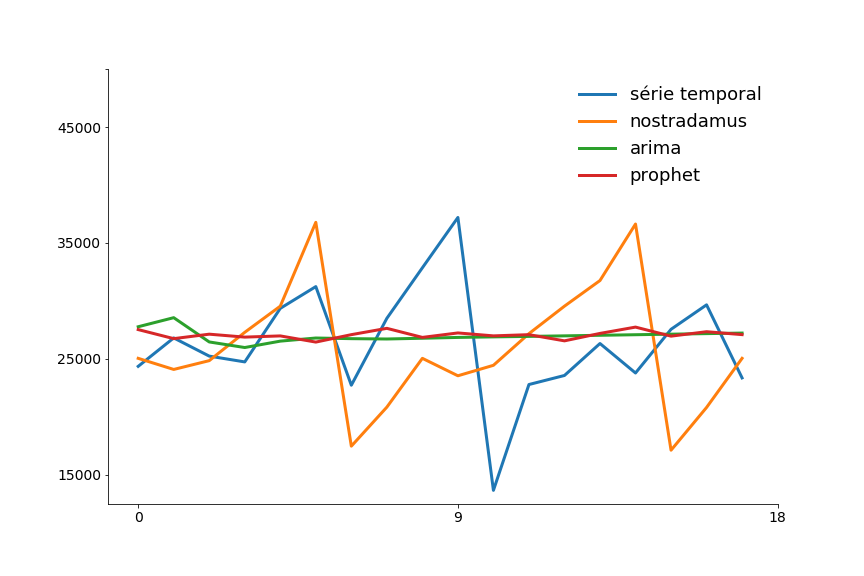
\includegraphics[scale=0.3]{fig2.png}
	\caption{Previsão de cada sistema na base \textit{wineind} nos 10\% da base reservados para teste}
	\label{fig2}
\end{figure}

Nota-se que, em geral, o sistema Nostradamus tenta ajustar os padrões de ambas as séries temporais, já o \textit{Prophet} e o \textit{ARIMA} acaba convergindo suas previsões em torno da média dos dados. Na figura \ref{fig1}, é possível ver que o sistema Nostradamus é bem sucedido no seu ajuste, pois obteve o menor erro médio e pode-se observar que segue o comportamento da série. Entretanto, na figura \ref{fig2}, apesar de relativamente seguir o padrão da série, o sistem faz isso de forma mais rápida do que as mudanças realmente ocorrem, o que acaba gerando uma previsão com erro maior do que a previsão "conservadora" da média dos dados.

\section{Conclusão}

Iniciamos o presente trabalho introduzindo alguns dos principais conceitos em relação a dados, a séries temporais e suas características, tipos de abordagens para sua modelagem, assim como a estruturação do presente trabalho. A seguir, expôs-se a forma do que chamou-se de abordagem da estatística inferencial a respeito da modelagem de séries temporais, conceitos como estacionariedade, tipos de processos, regressão espúria, processos de raiz unitária e uma explicação do modelo ARIMA. Posteriormente, expôs-se a forma do que chamou-se de abordagem da estatística preditiva no contexto geral de previsão, discutindo alguns dos principais algoritmos , como regressão linear, $k$ vizinhos próximos, árvore de decisão, máquinas de suporte de vetor e redes neurais profundas. Por fim, expôs-se uma proposta de sistema que automatiza a previsão de séries temporais que une conceitos de engenharia de características usando processos autorregressivos e algoritmos preditivos. Por fim, testamos o sistema proposto pelo presente trabalho comparando-o com outros dois algoritmos em sete bases de dados de séries temporais.

Verificou-se que o sistema proposto conseguiu atingir uma performance relativamente boa, alcançando o menor erro na base de teste em cinco das sete bases de dados, além de tentar prever, mesmo que não satisfatoriamente, o padrão das demais séries. O trabalho pode ser expandido de diversas formas: utilização de outras formas de pré processamento dos dados, como normalização, padronização, tomar o logarítmo da série; criação de outras características ligadas a sazonalidade e a temporalidade dos dados, como dia da semana, semana do ano, mês do ano no casa de dados diários, por exemplo; utilização de outros algoritmos preditivos, como redes neurais com estrutura \textit{Long Short-Term Memory}.


\begin{thebibliography}{99}
  \bibliographystyle{srt}

\bibitem{Gujarati} GUJARATI, D. N.; PORTER, D., \textit{Basic Econometrics}. 5ª ed. Nova Iorque: Mc Graw-Hill/Irwin, 2009.

\bibitem{Brockwell} BROCKWELL, P. J.; DAVID, R. A. \textit{Introduction to Time Series and Forecasting}. 3ª ed. Nova Iorque: Springer, 2016.

\bibitem{Hayashi} HAYASHI, F. \textit{Econometrics}. 1ª ed. Princeton: Princeton University Press, 2000.

\bibitem{Hamilton} HAMILTON, J. D. \textit{Time Series Analysis}. 1ª ed. Princeton: Princeton University Press, 1994.

\bibitem{Enders} ENDERS, W. \textit{Applied Econometric Time Series}. 4ª ed. Tuscaloosa: Wiley, 2014.

\bibitem{Greene} GREENE, W. H. \textit{Econometric Analysis}. 8ª ed. Nova Iorque: Pearson, 2018.

\bibitem{Hyndman} HYNDMAN, R. J., ATHANASOPOULOS, G. \textit{Forecasting: principles and practice}. 2ª ed. Monash: OTexts, 2018.

\bibitem{Yule} YULE, G. U. Why Do We Sometimes Get Nonsense Correlations Between Time Series? A study in sampling and the nature of time series. \textit{Journal of the Royal Statistical Society}, v. 89, p. 1-64, 1926.

\bibitem{Granger-Newbold} GRANGER, C. W. J.; NEWBOLD, P. Spurious Regressions in Econometrics. \textit{Journal of Econometrics}, v. 2, p. 111-120, 1974.

\bibitem{Dicker-Fuller} DICKEY, D. A.; FULLER, W. A. Distribution of the Estimators for Autorregressive Time Series with a Unit Root. \textit{Journal of American Statistical Association}, v. 74, p. 427-431, 1979.

\bibitem{Elliot-Rothenberg-Stock} ELLIOT, G.; ROTHENBERG, T. J.; STOCK, J. H. Efficient tests for an Autorregressive Unit Root. \textit{Econometrica}, v. 64, p. 813-836, 1996.

\bibitem{Phillips-Perron} PHILLIPS, P. C. B.; PERRON, P. Testing for a Unit Root in Time Series Regression. \textit{Biometrika}, v. 75, p. 335-346, 1988.

\bibitem{Kwiatkowski} KWIATKOWSKI, D. et al. Testing the Null Hypothesis of Stationarity Against the Alternative of a Unit Root. \textit{Journal of Econometrics}, v. 54, p. 159-178, 1992.

\bibitem{Brown} BROWN, R. G. \textit{Exponential Smoothing for Predicting Demand}. Cambridge: Arthur D. Little, 1956.

\bibitem{Holt} HOLT, C. C. Forecasting Trends and Seasonality by Exponentially Weighted Averages. \textit{Office of Naval Research Memorandum}, v. 52, 1957.

\bibitem{Winters} WINTERS, P. R. Forecasting Sales by Exponentially Weighted Moving Averages. \textit{Management Science}, v. 6, n. 3, p. 231-362, 1960.

\bibitem{Box-Jenkins} BOX, G. E. P.; JENKINS, G. M. \textit{Time Series Analysis: Forecasting and Control}. São Francisco: Holden-Day, 1976.

\bibitem{Ljung-Box} LJUNG, G. M.; BOX, G. E. On a Measure of Lack of Fit in Time Series Models. \textit{Biometrika}, v. 65, n. 2, p. 297-303, 1978.

\bibitem{Box-Pierce} BOX, G. E.; PIERCE, D. A. Distribution of Residual Autocorrelations in Autoregressive-Integrated Moving Average Time Series Models. \textit{Journal of the American Statistical Association}, v. 65, n. 332, p. 1509-1526, 1970.

\bibitem{Akaike} AKAIKE, H. A new look at the statistical model identification. \textit{IEEE Transactions on Automatic Control}, v. 19, n. 6, p. 716-723, 1974.

\bibitem{Schwarz} SCHWARZ, G. E. Estimating the dimension of a model. \textit{Annals of Statistics}, v. 6, n. 2, p. 461-464, 1978.

\bibitem{Hannan} HANNAN, E. J.; QUINN, B. G. The Determination of the Order of an Autoregression. \textit{Journal of the Royal Statistical Society}, v. 41, p. 190-195, 1979.

\bibitem{Oliver} OLIVER, T. \textit{Machine Learning for Absolute Beginners: a plain english introduction}. 1ª ed. Online: Theobald Oliver, 2017.

\bibitem{Laird} LAIRD, J. E.; NEWELL, A.; ROSENBLOOM, P. S. SOAR: an architecture for general intelligence. \textit{Artificial Intelligence}, v. 33, n. 1, p. 1-64, 1987.

\bibitem{Samuel} SAMUEL, A. Some Studies in Machine Learning Using the Game of Checkers. \textit{IBM Journal of Research and Development}, v. 3, n. 3, p. 210-229, 1959.

\bibitem{Kullbrack} KULLBRACK, S.; LEIBLER, R. A. On Information and Sufficiency. \textit{Annals of Mathematical Statistics}, v. 22, n. 1, p. 79-86, 1951.

\bibitem{James} JAMES, G. et al. \textit{An Introduction to Statistical Learning: with application in R}. Nova Iorque: Springer, 2013.

\bibitem{BreimanBag} BREIMAN, L. Bagging Predictors. \textit{Machine Learning}, v. 24, n. 2, p. 123-140, 1996.

\bibitem{BreimanRF} BREIMAN, L. Random Forests. \textit{Machine Learning}, v. 45, n. 1, p. 5-32, 2001.

\bibitem{BreimanB} BREIMAN, L. Arcing Classifier. \textit{Annals of Statistics}, v. 26, n. 3, p. 801–849, 1998.

\bibitem{Cortes} CORTES, C.; VAPNIK, V. N. Supporte-Vector Networks. \textit{Machine Learning}, v. 20, n. 3, p. 272-297, 1995.

\bibitem{Aizerman} AIZERMAN, M. A.; BRAVERMAN, E. M.; ROZONOER, L. I. Theoretical Foundations of the Potential Function Method in Pattern Recognition Learning. \textit{Automation and Remote Control}, v. 25, p. 821-837, 1964.

\bibitem{Hastie} HASTIE, T.; TIBSHIRANI, R.; FRIEDMAN, J. \textit{The Elements of Statistical Learning: data mining, inference and prediction}. 2ª ed. Nova Iorque: Springer, 2009.

\bibitem{Chen} CHEN, T.; GUESTRIN, C. (2016). XGBoost: A Scalable Tree Boosting System. In: \textit{Proceedings of the 22nd ACM SIGKDD International Conference on Knowledge Discovery and Data Mining}. São Francisco, CA, USA: ACM, 13-17 Agosto de 2016. p. 785–794. arXiv:1603.02754.

\bibitem{Pedregosa} PEDREGOSA, F. et al. Scikit-learn: Machine Learning in Python. \textit{Journal of Machine Learning Research}, v. 12, p. 2825-2830, 2011.

\bibitem{Lévesque} LÉVESQUE, J. C.; et al. Bayesian Optimization for Conditional Hyperparameter Spaces. In: \textit{2017 International Joint Conference on Neural Networks (IJCNN)}. IEEE, 2017. p. 286-293.

\end{thebibliography}

\end{document}
